\documentclass[12pt]{extarticle}
\usepackage{phys440}

\title{PHYS440 - Project: HHL Algorithm}
\author{John Hurst}
\date{June 2024}

\begin{document}
\maketitle

%%%%%%%%%%%%%%%%%%%%%%%%%%%%%%%%%%%%%%%%%%%%%%%%%%%%%%%%%%%%%%%%%%%%%%%%%%%%%%%%%%%%%%%%%%%%%%%%%%%%
\section{Introduction}

The Harrow-Hassidim-Lloyd (HHL) algorithm for solving linear systems\cite{hhl2009} is one of the first algorithms to promise a quantum speedup for a variety of real-world problems.
The walk-through in \cite{zaman2023step} shows the mathematics for each step and provides background on the relevant quantum computing concepts.
The paper gives a numerical example to illustrate the steps, and provides MATLAB and Qiskit code for the example.

For my PHYS440 project I studied the walkthrough to understand the HHL algorithm in some detail,
and supplemented this by reading several other introductory sources such as \cite{baaquie2023} and \cite{hidary2021}.

I ported the MATLAB sample code to two different Mathematica implementations.
The first implementation is a direct port of the matrix formulation of the circuit from MATLAB.
The second implementation uses the Wolfram Quantum Framework to implement the example using the QuantumCircuitOperator feature.

The paper's example uses a 2x2 matrix, and only two clock qubits, which does not sufficiently illustrate some features of the algorithm.
I created my own example with a 4x4 matrix and three clock qubits, to study these features in more detail.

I verified my example in Mathematica, and in a Qiskit program run on the IBM Quantum simulator.
I then created a more general Qiskit program to explore the behaviour and limits of the algorithm with larger matrices and more clock qubits.

I followed up with some more reading on the limits and applicability of HHL, starting from Aaronson's well-known paper \cite{aaronson2015read}.

The remainder of this report is in several parts.
\begin{itemize}
\item Part \ref{sec:implementation} discusses implementation details of the more general 4x4 numerical example, in particular the handling of the ancilla rotation.
\item Part \ref{sec:generalization} describes some experiments with larger systems and more clock qubits.
\item Part \ref{sec:applications} discusses the applicability of the HHL algorithm to real-world problems.
\end{itemize}

\section{Implementation Notes}\label{sec:implementation}

This report will not repeat all the details from \cite{zaman2023step}.
I will focus instead on what I found by generalising the example to a larger matrix and number of clock qubits.

\subsection{Example 4x4 problem}

For the sample problem, I constructed a 4x4 Hermitian matrix with ``friendly'' eigenvalues in ratio 1:2:3:4,
so that they could be represented exactly using 3 clock qubits.

I defined the matrix like this:
\begin{equation}\label{eq:matrixa4}
A = H_4 \begin{pmatrix}
    \frac{1}{3} & 0 & 0 & 0 \\
    0 & \frac{2}{3} & 0 & 0 \\
    0 & 0 & 1 & 0 \\
    0 & 0 & 0 & \frac{4}{3}
\end{pmatrix} H_4^{\dagger}
= \begin{pmatrix}
    \frac{5}{6} & -\frac{1}{3} & 0 & -\frac{1}{6} \\
    -\frac{1}{3} & \frac{5}{6} & -\frac{1}{6} & 0 \\
    0 & -\frac{1}{6} & \frac{5}{6} & -\frac{1}{3} \\
    -\frac{1}{6} & 0 & -\frac{1}{3} & \frac{5}{6}
\end{pmatrix}
\end{equation}
where $H_4$ is a 4x4 Hadamard matrix.
(There are different possible 4x4 Hadamard matrices, and a common choice is $H_4=H_2\otimes H_2$, but I used Mathematica's \texttt{HadamardMatrix[4]}, which is different.)

For $b$ I used
\begin{equation}\label{eq:vectorb4}
b = \begin{pmatrix} 1 \\ 2 \\ 3 \\ 2 \end{pmatrix}
\end{equation}

The solution is given by
\begin{equation}\label{eq:solutionx4}
A^{-1}b = \frac{1}{4}\begin{pmatrix} 19 \\ 23 \\ 29 \\ 25 \end{pmatrix}
\end{equation}
In the HHL algorithm with solution is scaled because it is read from the relative frequencies of different measurements.
For the purpose of checking the algorithm we'll use a scaled solution such that the elements sum to 1:
\begin{equation}\label{eq:solutionx4num}
x = \begin{pmatrix} 0.1979 \\ 0.2396 \\ 0.3021 \\ 0.2604 \end{pmatrix}
\end{equation}

\subsection{Circuit details}

My HHL circuit for a 4x4 matrix and three clock qubits is shown in Figures \ref{fig:circuit1}-\ref{fig:circuit3}.
The first register, labelled $b$, with two qubits, begins with the input state, and carries the result $x$ at the end.
The second register, labelled $q$, with three qubits, is the clock register.
The third register, labelled $a$, with one qubit, is the ancilla register.

Figure \ref{fig:circuit1} shows the state preparation and QPE.
Because the goal of my implementation is to understand the algorithm,
not to provide a practical implementation, I have provided the input state directly in Mathematica using the \texttt{QuantumTensorProduct[]} function:
\begin{lstlisting}[language=Mathematica]
psi1 =
    QuantumTensorProduct[
        Join[{QuantumState[Normalize[b]]},
              ConstantArray[QuantumState[{1, 0}], n + 1]]]
\end{lstlisting}
\begin{figure}[h]
\centering
$\begin{array}{c}
\Qcircuit @C=.5em @R=.8em {
\lstick{a}   & \qw & \qw      & \qw       & \qw & \qw & \qw & \qw & \qw & \qw & \qw & \qw & \qw & \qw & \qw \\
& & & & & & & \mbox{IQFT} & & & & & & & \\
\lstick{q_0} & \qw & \gate{H} & \ctrl{3} & \qw & \qw & \qswap & \gate{H} & \ctrl{1} & \qw & \ctrl{2} & \qw & \qw & \qw & \qw \\
\lstick{q_1} & \qw & \gate{H} & \qw & \ctrl{2} & \qw & \qw & \qw & \gate{R_{-1/2}} & \gate{H} & \qw & \ctrl{1} & \qw & \qw & \qw \\
\lstick{q_2} & \qw & \gate{H} & \qw & \qw & \ctrl{1} & \qswap \qwx[-2] & \qw & \qw & \qw & \gate{R_{-1/4}} & \gate{R_{-1/2}} & \gate{H} & \qw & \qw \\
\lstick{b_0} & \multigate{1}{\text{prepare } b} & \qw & \multigate{1}{U} & \multigate{1}{U^2} & \multigate{1}{U^4} & \qw & \qw & \qw & \qw & \qw & \qw & \qw & \qw & \qw \\
\lstick{b_1} & \ghost{\text{prepare } b} & \qw & \ghost{U} & \ghost{U^2} & \ghost{U^4} & \qw & \qw & \qw & \qw & \qw & \qw & \qw & \qw & \qw
\gategroup{2}{7}{5}{13}{1.4em}{--}
}
\end{array}$
\caption{State preparation and QPE}
\label{fig:circuit1}
\end{figure}
In real world applications, state preparation is a nontrivial problem, as discussed in \cite{aaronson2015read} and \cite{hhl2009}.

This part of the circuit is conceptually the same as in \cite{zaman2023step},
but because there are four values in the input $b$ and four unknowns in $x$, the unitary operation in the QPE has two target qubits instead of one.
Also, because there are three clock qubits, in QPE we apply $U$, $U^2$ and $U^4$, and the IQFT subcomponent is extended to three qubits.

Figure \ref{fig:circuit2} shows the ancilla rotation.
\begin{figure}[h]
\centering
$\begin{array}{c}
\Qcircuit @C=.5em @R=.8em {
\lstick{a}   & \qw & \gate{RY(\theta_1=2\inv{\sin}\frac{1}{4})} & \gate{RY(\theta_2=2\inv{\sin}\frac{1}{3})} & \gate{RY(\theta_3=\frac{\pi}{3})} & \gate{RY(\theta_4=\pi)} & \qw \\
\lstick{q_0} & \qw & \ctrlo{-1} & \ctrl{-1}  & \ctrlo{-1} & \ctrl{-1}  & \qw \\
\lstick{q_1} & \qw & \ctrlo{-2} & \ctrl{-2}  & \ctrl{-2}  & \ctrlo{-2} & \qw \\
\lstick{q_2} & \qw & \ctrl{-3}  & \ctrlo{-3} & \ctrlo{-3} & \ctrlo{-3} & \qw \\
% \lstick{b_0} & \qw & \qw & \qw & \qw & \qw & \qw \\
% \lstick{b_1} & \qw & \qw & \qw & \qw & \qw & \qw \\
}
\end{array}$
\caption{Ancilla rotation}
\label{fig:circuit2}
\end{figure}

This part of the circuit is the most interesting part of the project.

As discussed in class, I was confused about the number of rotations on the ancilla qubit.
In \cite{zaman2023step} there are two rotations on the ancilla qubit, using angles $\theta_1$ and $\theta_2$, and controlled by the two clock qubits.
The angles $\theta_1$ and $\theta_2$ are calculated from the eigenvalues of the matrix $A$.
So it was unclear to me whether there should be a distinct rotation were per eigenvalue, or per clock qubit.
It seemed to me from the construction of the circuit that it must be a rotation per clock qubit.
And also, in real-world applications we might have billions of unknowns and eigenvalues, but we will always have a fairly limited number of clock qubits, determined by the precision desired.
So it seemed to me that it would not be practical to consider rotations per eigenvalue.

It turns out that my thinking was not correct.
The rotations on the ancilla qubit achieve the inversion of the eigenvalues,
and so to get a solution with perfect accuracy it is necessary to have a rotation per eigenvalue.
However, in real world implementations, it's unlikely this would actually be done for large numbers of input qubits.
By being selective and careful about the rotations, an approximate solution satisfies the accuracy bounds in \cite{hhl2009}.
A recent paper, \cite{morgan2024enhanced}, discusses filtering rotations ``by relevance'' to maintain circuit depth advantages.

In the circuit in Figure \ref{fig:circuit2}, I have implemented four rotations with angles $\theta_1$, $\theta_2$, $\theta_3$ and $\theta_4$,
which correspond precisely to the eigenvalues $\lambda_1$, $\lambda_2$, $\lambda_3$ and $\lambda_4$ of the matrix $A$.
They are controlled by the clock qubits according to the binary representation of the eigenvalue phases on the clock qubits.
So for example, the first eigenvalue is $\lambda_1=\frac{4}{3}$.
In the Hamiltonian $e^{i\Lambda t}$ this eigenvalue has corresponding value $e^{i\lambda_1t}=e^{i\frac{4}{3}\times\frac{3\pi}{4}}=e^{2\pi i \frac{1}{2}}$.
Therefore the phase for this eigenvalue is $\phi_1=\frac{1}{2}$, which in binary is 0.100b.
Therefore the rotation for this eigenvalue should occur when qubit $q_2$ is set and qubits $q_1$ and $q_0$ are not set.
The rotation angle is obtained via the formula from \cite{zaman2023step}: $\theta_1=2\inv{\sin}\bar{\lambda}_1$,
where $\bar{\lambda}_1$ is the eigenvalue scaled by a factor that makes all the eigenvalues integers:
\[
\bar{\lambda_j}=\frac{2^n\lambda_jt}{2\pi}
\]
In this way we obtain the phases, controlling qubits, and rotation angles for all the eigenvalues, shown in the table below:
\begin{center}
\begin{tabular}{|c|c|c|c|c|}
\hline
Eigenvalue & $e^{i\lambda t}=e^{2\pi i\phi}$ & Phase & Qubits & Angle \\
\hline
$\lambda_1=\frac{4}{3}$ & $e^{i\lambda_1t}=e^{i \frac{4}{3} \times \frac{3\pi}{4}}=e^{2\pi i \frac{1}{2}}$ & $\phi_1=\frac{1}{2}=$0.100b & $q_2\overline{q_1}\overline{q_0}$ & $\theta_1=2\inv{\sin}\frac{1}{4}$ \\
$\lambda_2=1$           & $e^{i\lambda_2t}=e^{i 1 \times \frac{3\pi}{4}}=e^{2\pi i \frac{3}{8}}$   & $\phi_2=\frac{3}{8}=$0.011b & $\overline{q_2}q_1q_0$ & $\theta_2=2\inv{\sin}\frac{1}{3}$ \\
$\lambda_3=\frac{2}{3}$ & $e^{i\lambda_3t}=e^{i \frac{2}{3} \times \frac{3\pi}{4}}=e^{2\pi i \frac{1}{4}}$ & $\phi_3=\frac{1}{4}=$0.010b & $\overline{q_2}q_1\overline{q_0}$ & $\theta_3=2=2\inv{\sin}\frac{1}{2}=\frac{\pi}{3}$ \\
$\lambda_4=\frac{1}{3}$ & $e^{i\lambda_4t}=e^{i \frac{1}{3} \times \frac{3\pi}{4}}=e^{2\pi i \frac{1}{8}}$ & $\phi_4=\frac{1}{8}=$0.001b & $\overline{q_2}\overline{q_1}q_0$ & $\theta_4=2=2\inv{\sin}\frac{1}{1}=\pi$ \\
\hline
\end{tabular}
\end{center}
The controlling qubits and rotation angles correspond to the circuit portion in Figure \ref{fig:circuit2}.
% TODO: How might this have been shown more clearly in zaman2023step?

Figure \ref{fig:circuit3} shows the reverse QPE and measurement.
As in \cite{zaman2023step}, if the ancilla qubit is measured in state $\ket{1}$,
then the $b$ register holds the correct $x$ result.
If the ancilla qubit is measured in state $\ket{0}$, the result is discarded and the circuit must be run again.
\begin{figure}[h]
\centering
$\begin{array}{c}
\Qcircuit @C=.4em @R=.7em {
    \lstick{a}   & \qw & \qw & \qw & \qw & \qw & \qw & \qw & \qw & \qw & \qw & \qw & \qw & \meter \\
    & & & \mbox{QFT} & & & & & & & & & & & & \\
    \lstick{q_2} & \qw & \qw & \qw & \ctrl{2} & \qw & \ctrl{1} & \gate{H} & \qswap & \qw & \qw & \ctrl{3} & \gate{H} & \qw \\
    \lstick{q_1} & \qw & \qw & \ctrl{1} & \qw & \gate{H} & \gate{R_{1/2}} & \qw & \qw & \qw & \ctrl{2} & \qw & \gate{H} & \qw \\
    \lstick{q_0} & \qw & \gate{H} & \gate{R_{1/2}} & \gate{R_{1/4}} & \qw & \qw & \qw & \qswap \qwx[-2] & \ctrl{1} & \qw & \qw & \gate{H} & \qw \\
\lstick{b_0} & \qw & \qw & \qw & \qw & \qw & \qw & \qw & \qw & \multigate{1}{U^{-4}} & \multigate{1}{U^{-2}} & \multigate{1}{U^{-1}} & \qw & \meter \\
\lstick{b_1} & \qw & \qw & \qw & \qw & \qw & \qw & \qw & \qw & \ghost{U^{-4}} & \ghost{U^{-2}} & \ghost{U^{-1}} & \qw & \meter
\gategroup{2}{3}{5}{8}{1.4em}{--}
}
\end{array}$
\caption{Inverse QPE and measurement}
\label{fig:circuit3}
\end{figure}

% \begin{figure}[H]
% \centering
% 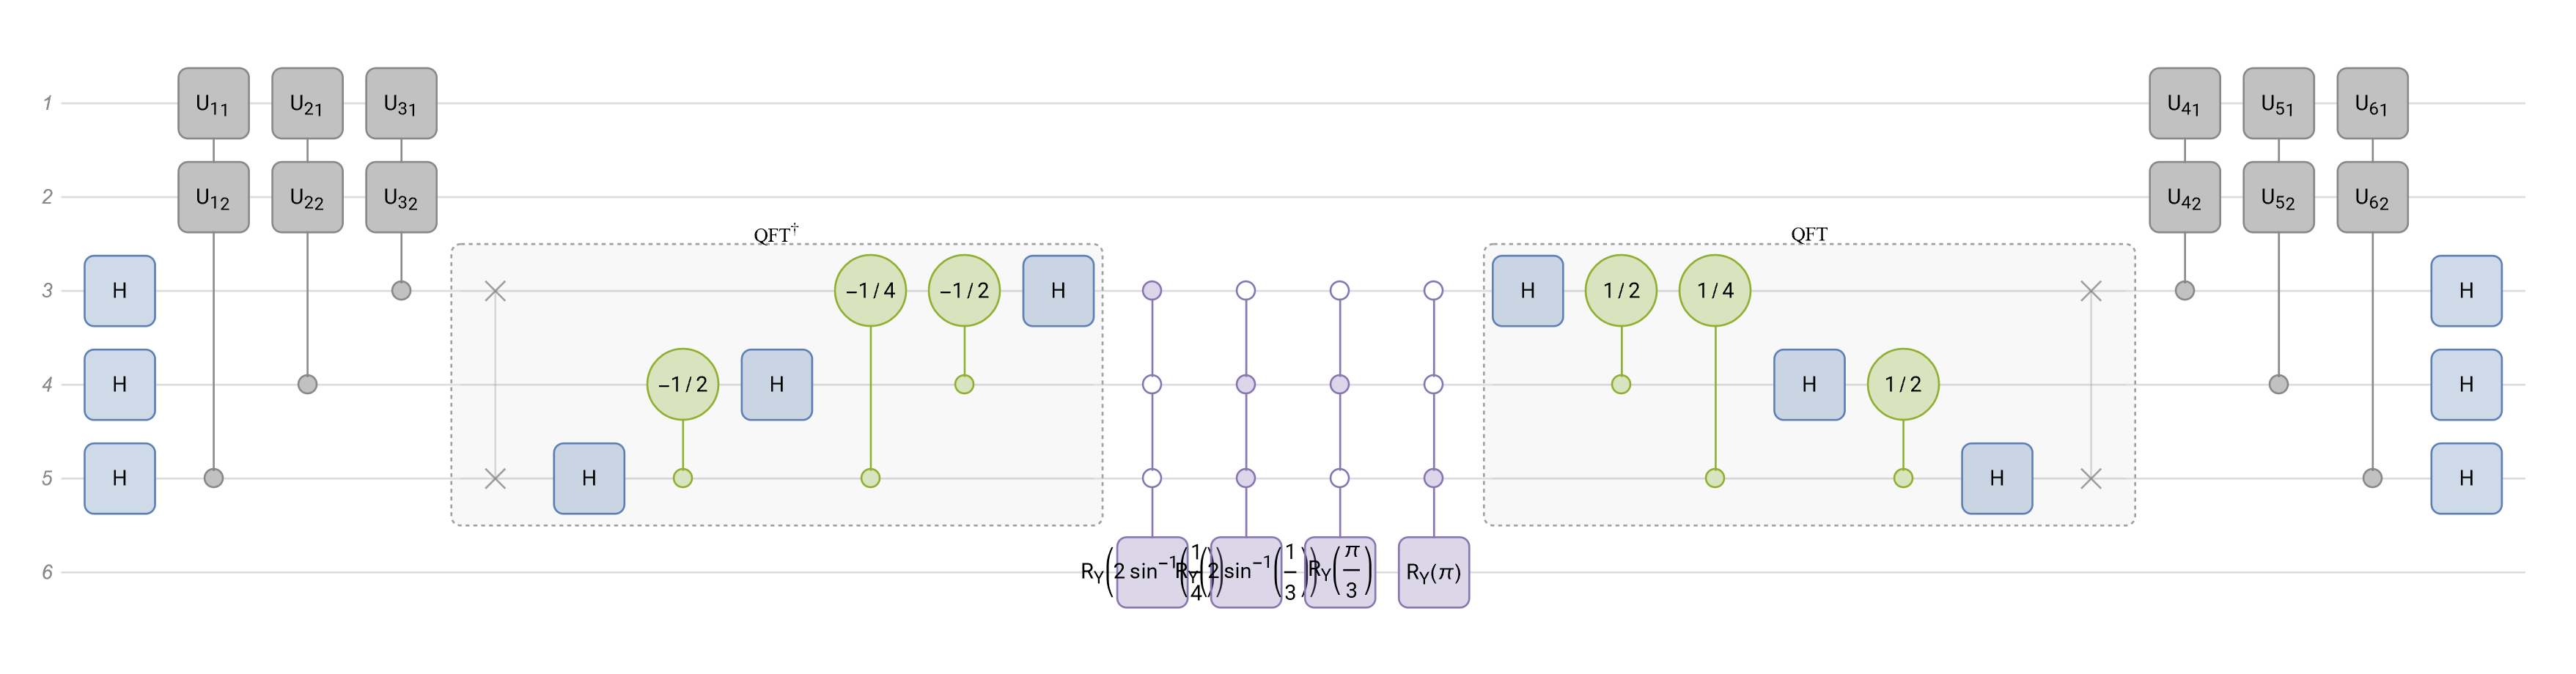
\includegraphics[width=0.80\textwidth]{images/project_hhl_4x4_mathematica.png}
% \caption{Mathematica circuit for 4x4 problem}
% \label{fig:hhl_4x4_mathematica}
% \end{figure}

\subsection{Qiskit circuit implementation}

I wrote a Qiskit program to construct the circuit for the 4x4 problem and run it on the IBM Quantum simulator.
A sample run looks like this:

\begin{lstlisting}[language=Bash]
bin/project_hhl_4x4_qiskit.py --shots=10000 --filename=project_hhl_4x4.png
000000  434
000001  1345    0.1476  0.1944
010000  1
010001  2053    0.2252  0.2402
100000  450
100001  3274    0.3592  0.3033
110001  2443    0.2680  0.2620
Prob(ancilla |0>) = 0.9115
\end{lstlisting}

The first part of the output is a table in four columns:
\begin{itemize}
\item The measurement bits: $b_1$, $b_0$, $q_2$, $q_1$, $q_0$, $a$.
\item The number of times that measurement was observed (the count).
\item The frequency of that measurement: count/total.
\item The square root of the frequency, corresponding to the estimate for the corresponding $x$.
\end{itemize}

Measurements with the ancilla bit (the least significant, or rightmost bit in the output) having value 1 are counted in the result,
and measurements with the ancilla bit having value 0 are discarded.

Following this table is the frequency that the ancilla bit was measured in state $\ket{0}$ (having value 1), in this case 0.9115,
indicating a good effectiveness for the algorithm with these data.

The output from this run is shown more clearly in table \ref{tab:results4x4}, along with the actual $x$ values for comparison.
We can see from the results that with 10,000 shots, we have got pretty good estimates for $x$.

\begin{table}[h]
\begin{center}
\begin{tabular}{|c|r|r|r|r|}
\hline
Measurement & Count & Frequency & $x$ estimate & $x$ actual \\
\hline
000000 &  434 & & & \\
000001 & 1345 & 0.1476 & 0.1944 & 0.1979 \\
010000 &    1 & & & \\
010001 & 2053 & 0.2252 & 0.2402 & 0.2396 \\
100000 &  450 & & & \\
100001 & 3274 & 0.3592 & 0.3033 & 0.3021 \\
110001 & 2443 & 0.2680 & 0.2620 & 0.2604 \\
\hline
\end{tabular}
\caption{Results for 4x4 system}
\label{tab:results4x4}
\end{center}
\end{table}

Figure \ref{fig:hhl_4x4_qiskit} shows the Qiskit circuit for the 4x4 problem.
\begin{figure}[H]
\centering
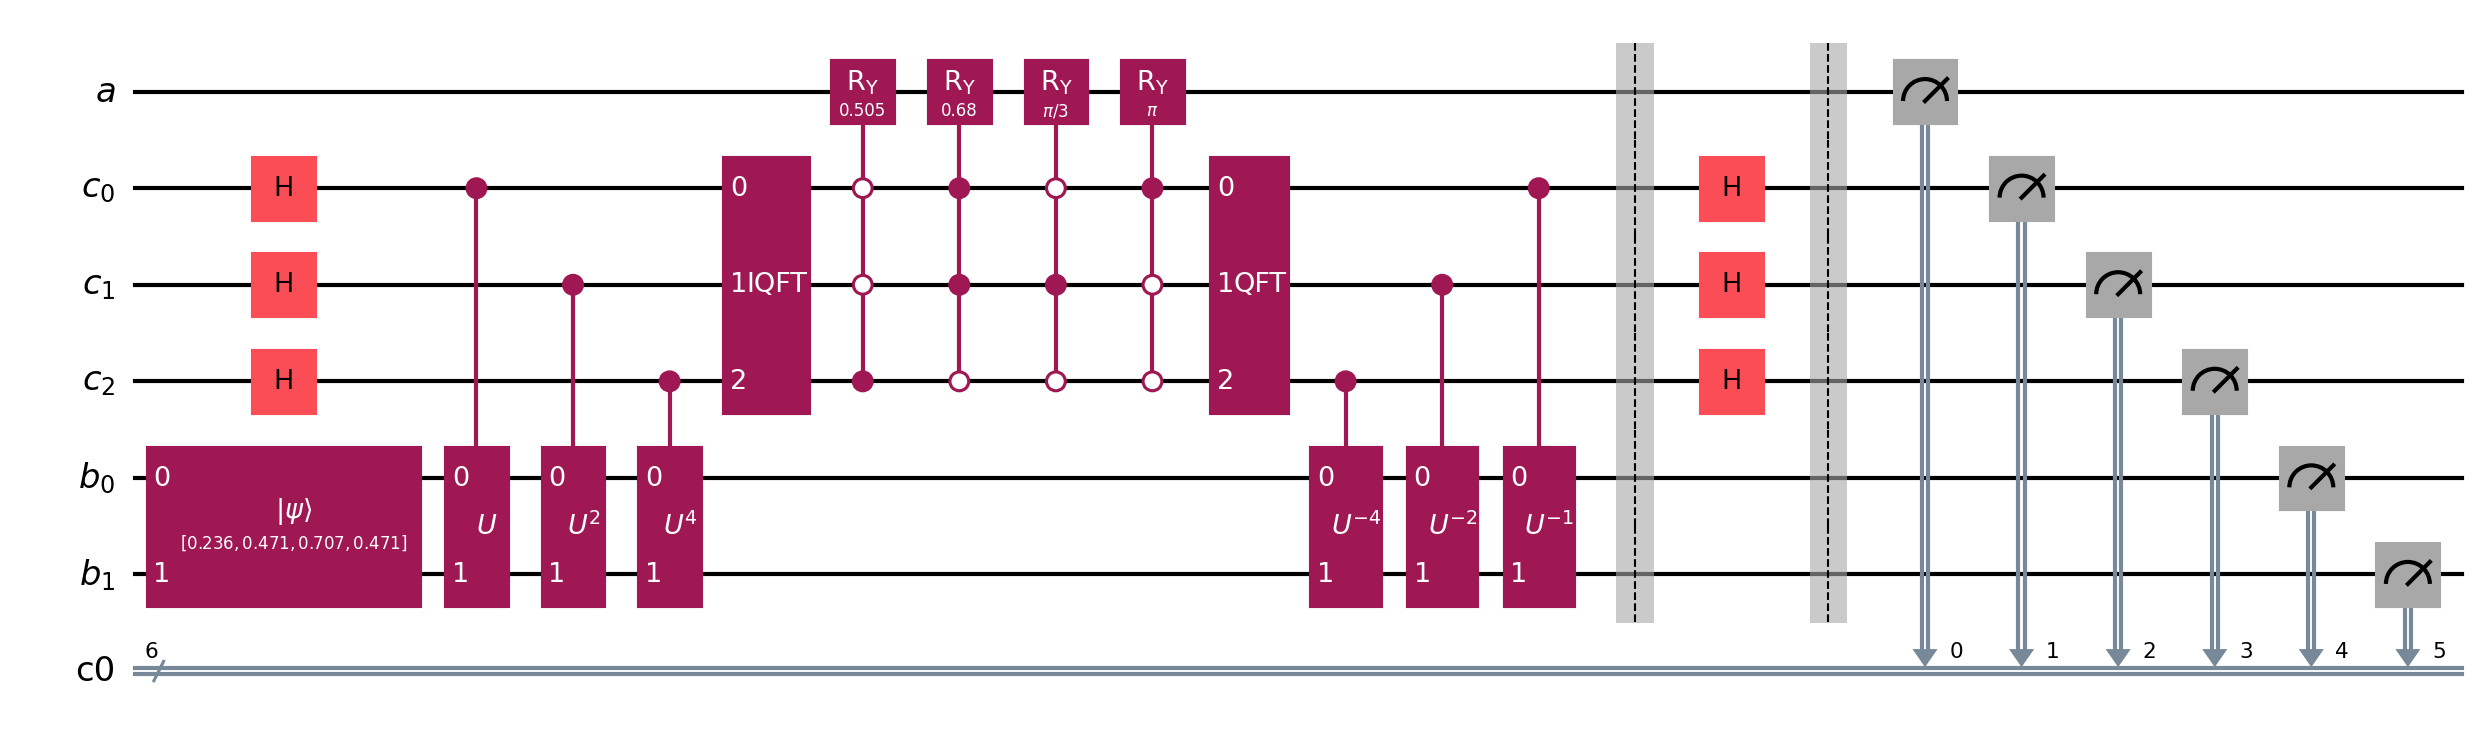
\includegraphics[width=0.80\textwidth]{images/project_hhl_4x4.png}
\caption{Qiskit circuit for 4x4 problem}
\label{fig:hhl_4x4_qiskit}
\end{figure}

\section{Generalization}\label{sec:generalization}

I created a more general Qiskit program to explore the behaviour and limits of the algorithm with larger matrices and more clock qubits.
I also created an 8x8 Hermitian matrix using a similar procedure to above.
This Qiskit program prints the actual $x$ solution values (scaled appropriately), as well as the estimates, to make comparison easier.

For the 8x8 example I ran the program as follows:
\begin{lstlisting}[language=Bash]
bin/project_hhl_qiskit.py --shots=1000000 --clockqubits=6 \
    data/project_hhl/Ahalf_8x8.csv data/project_hhl/b_8x8.csv
\end{lstlisting}

The output is shown in table \ref{tab:results8x8}.

\begin{table}[h]
\begin{center}
\begin{tabular}{|c|r|r|r|r|}
\hline
Measurement & Count & Frequency & $x$ estimate & $x$ actual \\
\hline
0000000000  &  11019 & & & \\
0000000001  &     26 & 0.0000 & 0.0091 & 0.0091 \\
0010000000  &  77671 & & & \\
0010000001  &    609 & 0.0006 & 0.0440 & 0.0435 \\
0100000000  &  80853 & & & \\
0100000001  &  10871 & 0.0109 & 0.1859 & 0.1858 \\
0110000000  &  12558 & & & \\
0110000001  &    451 & 0.0005 & 0.0379 & 0.0377 \\
1000000000  & 230535 & & & \\
1000000001  &   4079 & 0.0041 & 0.1139 & 0.1141 \\
1010000000  &  50226 & & & \\
1010000001  &    370 & 0.0004 & 0.0343 & 0.0329 \\
1100000000  & 110700 & & & \\
1100000001  &   6789 & 0.0068 & 0.1469 & 0.1476 \\
1110000000  & 345591 & & & \\
1110000001  &  57652 & 0.0577 & 0.4281 & 0.4293 \\
\hline
\end{tabular}
\caption{Results for 8x8 system}
\label{tab:results8x8}
\end{center}
\end{table}

The frequency of the ancilla bit being measured in state $\ket{0}$ was only 0.0808, which is why I needed to run with 1,000,000 shots to get an accurate result.
The fact that the result was correct, yet the ancilla frequency is so low, is troubling.
I tried several things to understand the cause of this:
\begin{itemize}
\item Ensure the matrix is well-conditioned, as described in \cite{hhl2009}.
\item Ensure the matrix is sparse.
\item Construct a Hermitian matrix more directly as two blocks of a a 4x4 matrix and its conjugate transpose.
\end{itemize}
None of these measures made much difference to results: the $x$ estimate was always good, but the ancilla frequency was always low.

I also tried two variations of the eigenvalue scaling and clock qubit arrangement.
In my default setup I scale the eigenvalues so that the largest one is scaled to $\frac{1}{2}$=0.100... (base 2), following the example in \cite{zaman2023step}.
But this is wasteful, because it effectively reduces the range of values that can be represented by the clock qubits by half.
So I tried another scheme where I scaled so that the largest eigenvalue is scaled to $0.111...$ (base 2), making maximum use of the clock qubits.
(For this I needed to use a different input matrix, chosen to make the eigenvalue ratios fit the clock qubit scheme.)

Because none of these approaches resulted in a good value for the ancilla frequency, I suspect that there may be one or more buggs remaining in my implementation.

TODO: Histogram of ancilla values for random 4x4 problems.

TODO: Chi-square tests of observed frequencies for random problems, 4x4 and 8x8.

\section{Applications}\label{sec:applications}

\printbibliography
\addcontentsline{toc}{section}{References}


\end{document}
